% Five sources of variation in a model call, and what to do about each.
% ---------------------------------------------------------------------------
% style.tex --- shared preamble for every figure in book/figures/tikz/
%
% One style for all figures: Latin Modern, thin black lines, a light grey
% fill, and one accent colour used only to mark what is untrusted or wrong.
% Build with scripts/build_figures.sh; see book/figures/README.md.
% ---------------------------------------------------------------------------
\documentclass[tikz,border=6pt]{standalone}
\usepackage[T1]{fontenc}
\usepackage{lmodern}
\usetikzlibrary{arrows.meta,positioning,shapes.geometric,calc,fit,backgrounds}

\hyphenpenalty=10000   % short lines in boxes: ragged, never hyphenated

\definecolor{lightgrey}{gray}{0.92}
\definecolor{accent}{HTML}{9B2D20}

\tikzset{
  every picture/.style={
    line width=0.6pt,
    font=\small,
    >={Stealth[length=5pt,width=4pt]},
    node distance=14pt and 24pt,
  },
  % shapes
  box/.style={draw, rectangle, inner xsep=8pt, inner ysep=5pt,
              minimum height=22pt, align=center},
  grey/.style={box, fill=lightgrey},
  rounded/.style={box, rounded corners=9pt},
  decision/.style={draw, diamond, aspect=2.4, inner sep=1.5pt, align=center},
  group/.style={draw, dashed, rounded corners=5pt, inner sep=7pt},
  % text
  tag/.style={font=\footnotesize, align=center, inner sep=2pt},
  note/.style={font=\footnotesize\itshape, align=center, inner sep=2pt},
  code/.style={font=\small\ttfamily},
  codetag/.style={font=\footnotesize\ttfamily, align=center, inner sep=2pt},
  title/.style={font=\small\scshape, align=center, inner sep=2pt},
  % lines
  arrow/.style={->},
  back/.style={->, dashed},
  thin/.style={line width=0.4pt, gray},
  % the one accent, for what is untrusted, wrong or missing
  bad/.style={accent},
  badbox/.style={box, draw=accent, text=accent},
}

\begin{document}
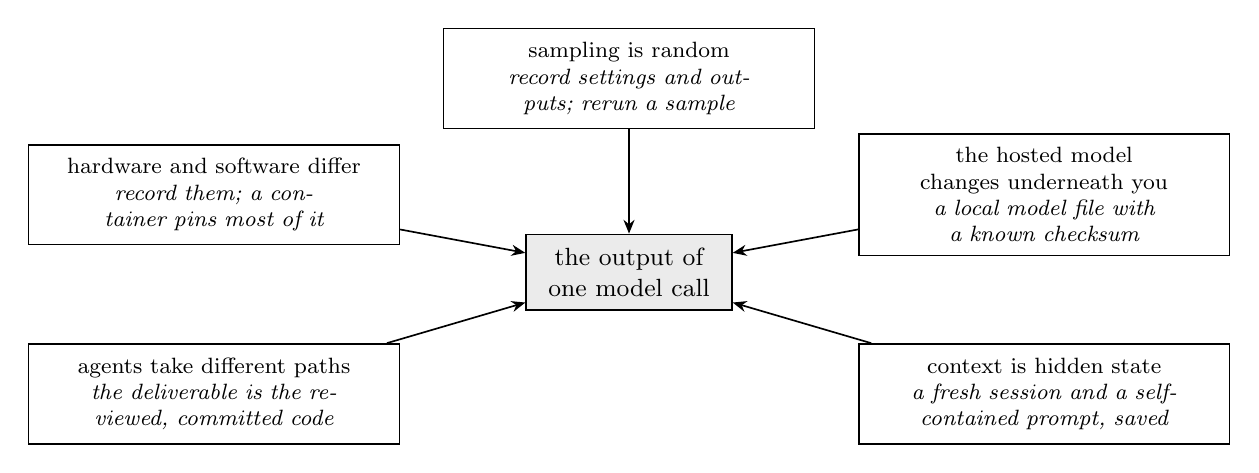
\begin{tikzpicture}[src/.style={box, text width=118pt, align=center, font=\footnotesize}]
  \node[grey] (out) at (0,0) {the output of\\one model call};
  \node[src] (a) at (0,70pt) {sampling is random\\ \itshape record settings and outputs; rerun a sample};
  \node[src] (b) at (150pt,28pt) {the hosted model changes underneath you\\ \itshape a local model file with a known checksum};
  \node[src] (c) at (150pt,-44pt) {context is hidden state\\ \itshape a fresh session and a self-contained prompt, saved};
  \node[src] (d) at (-150pt,-44pt) {agents take different paths\\ \itshape the deliverable is the reviewed, committed code};
  \node[src] (e) at (-150pt,28pt) {hardware and software differ\\ \itshape record them; a container pins most of it};
  \foreach \n in {a,b,c,d,e} \draw[->] (\n) -- (out);
\end{tikzpicture}
\end{document}
